\chapter{SL = L: Undirected connectivity in Logspace}

\section{Computing Resources}
Four main computing resources that we consider as limited (and measure the performance of our algorithms against)
\begin{itemize}
	\item Time 
	\item Memory
	\item Randomness
	\item Communication
\end{itemize}

\section{Problem Statement}

\begin{itemize}
	\item \textbf{Input}: Graph $G = (V, E)$; with source and target marked as $s, t$
	\item \textbf{Output}: YES iff $s$ and $t$ are connected, NO otw.
\end{itemize}

Above is the ``traditional'' definition of $s-t$ connectivity which we can solve with a vanilla BFS or DFS. This will take $\mathcal O ( |V| + |E| ) $ and $\mathcal O (|V| )$ extra bits of space / memory. The question is then, can we solve the same problem with sub-linear extra memory usage. 

\begin{proposition}
	There is a randomized algorithm with $5 \log |V|$ bits of additional memory (directed and undirected graphs). 
\end{proposition}

\begin{proposition}[Omer Reingold, 2005]
	There is a log space ($\mathcal O ( \log | V | )$) algorithm \textbf{(deterministic)} for undirected graphs. \footnote{first great hit ...}
\end{proposition}

It is yet unknown if we can achieve log space for directed graphs (with deterministic algorithm). The best known algorithms runs with $\mathcal O (\log |V| ) ^{3/2}$ bits of memory. Why is this so challenging? 

\begin{proposition}
	If divided $s-t$ connectivity can be solved with $\mathcal O (\log |V| )$ extra bits of memory (without randomness), then any randomized algorithm can be made deterministic at the expenses of a constant factor increase in memory. 
\end{proposition}

\subsection{Log Space USTCON - Results}
Here we highlight the progression in space complexity in various papers
\begin{itemize}
	\item \textbf{Nisan, 92}: Space $\mathcal O (\log ^ 2 N)$, time $N ^{\mathcal O (1)}$ algorithm... improved to $\mathcal O (\log ^ {4/3} N)$ in space. 
	\item \textbf{Reingold, 05}: Space $\mathcal O (\log N)$, time $N ^{\mathcal O (1)}$ algorithm. 
	\item \textbf{Trifornov, 05}: Space $\mathcal O ((\log N )(\log\log N))$ algorithm. 
\end{itemize}

\section{Randomized Algorithm for Connectivity}
\begin{algorithm}[Random Walk Algorithm for Connectivity] Here is the algorithm
	\begin{itemize}
		\item $steps \gets 0 $ 
		\item $current \gets s$; $target \gets t$
		\item while $steps < T$
		\begin{itemize}
			\item $current \gets $ random neighbor of current
			\item if $current == target$ return $YES$
		\end{itemize}
		\item return $NO$
	\end{itemize}
\end{algorithm}
The total memory for this algorithm is 
\begin{equation}
	2 \log N + \log T \leq 5 \log N
\end{equation}
extra bits, assuming we can get random neighbor. 

\begin{proposition}[Alenilaus, 80s]
	If $T = 100N^3$ steps, then $Pr$[Algorithm wrong] < $\frac{1}{3}$
\end{proposition}
which can improved to arbitrary accuracy by repeating the algorithm. Algorithms of this nature can perform bad on graphs known as ``Lollipop Graphs'' and even worse a ``Dumbell Graph''


\section{Spectral Graph Theory}
Consider an undirected graph $G = (V, E)$, 
\begin{definition}[Degree]
	Degree of a vertex $v$ is the number of edges $v$ is connected to.
\end{definition}

\begin{definition}[Regular]
	Graphs is ``regular'' if all vertices have same degree. 
\end{definition}

\begin{definition}[Adjacency Matrix]
	$A(G)$ is a symmetric matrix where $A(G)_{ij}$ = 1 if $\{i, j\}$ is an edge, 0 otw. 
\end{definition}

\begin{definition}[Normalized Adj Matrix]
	If $G$ is regular and has degree $D$, then the normalized adjacency matrix is defined as 
	\begin{equation}
		M(G) \equiv \frac{A(G)}{D}
	\end{equation}
\end{definition}

\begin{lemma}
	If $G$ is regular, then $1$ is an eigenvalue of $M(G)$. And $\bv_1 = \begin{bmatrix}
		1 & 1 & \dots & 1
	\end{bmatrix}^\top$ is an eigenvector with eigenvalue 1. 
\end{lemma}

\begin{proposition}[Eigenvalues of Regular Graphs]
	\label{prop:eigenvalues_of_regular_graphs}
	If $G$ is regular, then all eigenvalues of $M(G)$ have magnitude $\leq 1$. 
\end{proposition}

\begin{proof}
	WLOG assume $x_3$ is the largest entry in the vector $\bx$, then
	\begin{align}
		\lambda |x_3| 
		&= |M_{31}x_1 + M_{32}x_2 + ... + M_{3N}x_N| \\
		&\leq M_{31}|x_3| + M_{32}|x_3| + ... + M_{3N} |x_3| \\
		&= (M_{31} + \ldots + M_{3N}) |x_3| \\
		&= 1 |x_3|
	\end{align}
	Thus, $\lambda \leq 1$. \qed
\end{proof}

\begin{proposition}[Connectedness and Matrices]
	Regular $G = (V, E)$ is connected if and only if the only eigenvector with eigenvalue 1 for $M(G)$ is the all 1 vector. \footnote{i.e., eigenvalue 1 has an multiplicity of 1.}
\end{proposition}

\begin{proof} [Regular $G = (V, E)$ is connected implies $\lambda = 1$ has multiplicity of 1 for $M(G)$.]
	From proof to Prop. \ref{prop:eigenvalues_of_regular_graphs} we already know that $|\lambda| \leq 1$. With $x_j = \max(\bx)$ as the largest entry in the eigenvector, we recall (and abstract the inequality used back then as
	\begin{equation}
		|\lambda||x_j| = |(M(G)\bx)_j| = \left| \sum_{v_i \in N(v_j)} x_i \right| / D \leq |x_j| 
	\end{equation}
	We are now interested in the condition of when $\lambda = 1, |\lambda| |x_j| = |x_j|$, in which case we need 
	\begin{equation}
		x_i = x_j, \quad \forall v_i \in N(v_j)
	\end{equation}
	This suffices as a proof to every eigenvector with eigenvalue 1 to $M(G)$ is the $\mathbf 1$ vector. \qed
\end{proof}

\begin{proof} [$\lambda = 1$ has multiplicity of 1 for $M(G)$ implies regular $G = (V, E)$ is connected.]
	todo \dots
\end{proof}

\begin{proposition}[Eigenvalues of a Regular Graph]
	If $G$ is regular, then the eigenvalues of $M(G)$ are 
	\begin{equation}
		1 = \lambda_1 \geq \lambda_2 \geq \dots \geq \lambda_N
	\end{equation}
\end{proposition}

\begin{proof}
	This follows from the proof for Prop. \ref{prop:eigenvalues_of_regular_graphs} where we proved that all eigenvalues of $M(G)$ have magnitude $\leq$ 1. Since the one vector $\mathbf 1$ is an eigenvector of $M(G)$ with eigenvalue one, we know that $\lambda_1 = 1$ is attainable. This suffices as a proof. \qed
\end{proof}

\begin{proposition}
	$G$ is connected and regular if and only if on $M(G)$
	\begin{equation}
		\max ( |\lambda_2| , |\lambda_3|, \dots, |\lambda_N|) < 1
	\end{equation}
\end{proposition}

\begin{proof}
	todo ... 
\end{proof}

\begin{proposition}[Eigenvalues of D-Regular Graphs]
	If $G$ is a D-regular graph, then
	\begin{itemize}
		\item 1 is an eigenvalue of $M(G)$, and 
		\item all eigenvalues of $M(G)$ are at most 1 in absolute value
	\end{itemize}
\end{proposition}

\begin{definition}[Self Loops]
	We add connections from each node in the graph to themselves. In the matrix representation, we set $G_{ii} = 1, \forall i$. 
\end{definition}

\begin{definition}[Second Largest Eigenvalue]
	... denoted as $\lambda(G)$ or $\lambda_2(G)$. 
\end{definition}

\begin{lemma}
	If $G$ is D-regular and \textbf{has self loops}, then $G$ is connected if and only if $\lambda(G) < 1$.
\end{lemma}

\begin{proof} 
[$G$ is disconnected implies $\lambda(G) = 1$ (via contrapositive).] 
Consider a graph $G$ such that it is comprised of two clouds of disjoint graphs $G_1$ and $G_2$. Then the adjacency matrix of $G$ will take a block matrix form
\begin{equation}
	M_G = \begin{bmatrix}
		M_{G_1} & [\bzero ]  \\
		[\bzero ] & M_{G_2}
	\end{bmatrix}
\end{equation}
From linear algebra, we know that the eigenvalues of $M_G$ will be the union of eigenvalues of $M_{G_1}$ and $M_{G_2}$. Now, consider
\begin{equation}
	\bx^{(1)} = 
	\begin{bmatrix}
		1 \\ 1 \\ \vdots \\ 0 \\ 0
	\end{bmatrix} 
	\quad \quad \text{and} \quad \quad
	\bx^{(2)} = 
	\begin{bmatrix}
		0 \\ 0 \\ \vdots \\ 1 \\ 1
	\end{bmatrix}
\end{equation}
are both eigenvectors of $M_G$ with eigenvalues of 1. Hence, there are two orthogonal eigenvectors with eigenvalue 1, and $\lambda(G) = 1$ as wanted. 
\qed

\end{proof}

\begin{proof} [If $G$ is connected, then $\lambda(G) < 1$.] We already know that 1 is an eigenvalue of $M_G$ with the $\mathbf 1$ vector as eigenvector. Suppose $\lambda$ is also an eigenvalue with $\bv$ as an eigenvector and $\bv$ is perpendicular to $\mathbf 1$. Now, 
\begin{equation}
	\label{eq:eigenvector_perp_to_1}
	\mathbf 1 \perp \bv \implies \langle \bv, \mathbf 1 \rangle = v_1 + v_2 + \dots  + v_N  = 0
\end{equation}
The vector $\bv$ must contain some positive entries and some negative entries, we separate them into two sets
\begin{equation}
	P = \{ i : v_i \geq 0\} \quad \text{and} \quad N = \{ i : v_i < 0 \}
\end{equation}
where both sets are non-empty by Eq. \ref{eq:eigenvector_perp_to_1}. Taking a step back and reorganize the goal into matrix form
\begin{equation}
	M_G \begin{bmatrix}
		+ \\ + \\ \vdots \\ - \\ -
	\end{bmatrix} = \lambda \begin{bmatrix}
		+ \\ + \\ \vdots \\ - \\ -
	\end{bmatrix}\quad \quad \text{where} \quad \begin{bmatrix}
		+ \\ + \\ \vdots \\ - \\ - \end{bmatrix} = \begin{bmatrix}
			\mathbf P \\ - \\ \mathbf N
		\end{bmatrix} = \bv
\end{equation}
Per element, 
\begin{equation}
	\sum_{j = 1}^N M_G[i, j]\cdot v_j = \lambda \cdot v_i, \quad \forall i
\end{equation}
By the connectedness assumption, there must always be some edge connecting $P$ and $N$ the two sets, so
\begin{align}
	\lambda \left( \sum_{i \in P} v_i \right) 
	&= \sum_{i \in P} \left( \sum_{j = 1}^N M_G[i, j] \cdot v_j \right) \\
	&= \sum_{j = 1}^N v_j \sum_{i \in P} M_G[i, j] \\
	&= \sum_{j \in P} v_j \left( \sum_{i \in P} M_G[i, j] \right) + \sum_{j \in N} v_j \left( \sum_{i \in P} M_G[i, j] \right) \\
	&\leq \sum_{j \in P} v_j (1) + \sum_{j \in N} v_j \left( \sum_{i \in p} M_G[i, j] \right) \\
	&< \sum_{j \in P} v_j
\end{align}
where in the last two steps we utilized the facts that $M_G$'s columns add up to 1 and we have at least 1 non-zero entry in each row and col of $M_G$. 

In summary, we obtained
\begin{equation}
	\lambda \left( \sum_{i \in P} v_i \right) < \left( \sum_{j \in P} v_j \right) \quad \implies \quad \lambda < 1
\end{equation}
\qed

\end{proof}

\begin{definition}[Spectral Gap]
	Spectral Gap of a D-regular graph G is defined as 
	\begin{equation}
		\text{SpectralGap} (G) 
		\equiv 1 - \lambda(G)
	\end{equation}
\end{definition}

\begin{lemma}
	If $G$ is a D-regular connected graph with self-loops, then
	\begin{equation}
		\lambda (G) \leq 1 - \frac{1}{2D^2 \cdot N^2}
	\end{equation}
\end{lemma}

\begin{definition}
	We say a graph $G$ is $(N, D, \lambda)$ if it has $N$ vertices, $D$ regular and $\lambda(G) \leq \lambda$. 
\end{definition}


\section{Path Enumeration}
The simplest case is wen the shortest path between $s, t$ is short. Then, we can enumerate all paths of some length and see if $t$ is reached. 

The algorithm goes as follows
\begin{algorithm}
	1, Explore all paths of length less than or equal to $T$ from $s$. 2, If you reach $t$ in these explorations, output YES. If not, output NO. 
\end{algorithm}
This takes $\mathcal O (\log D) \cdot T$ extra space, where $D$ is the degree of the graph and $T$ is the loop times. 

\begin{definition}[Graph Diameter]
	Diameter of a graph is defined as the length of the longest shortest path for any pair of vertices. By convention, 
	\begin{itemize}
		\item G disconnected, diameter = $\infty$, and
		\item G connected, diameter = $\max_{i \neq j} \left( ShortestPath (i, j) \right)$
	\end{itemize}
\end{definition}

\begin{proposition}[Extra Space for Path Enumeration]
	Path enumeration will solve the $s-t$ connectivity in with max extra space 
	\begin{equation}
		(\log D) \cdot \Delta (G) \label{eq:path_enumeration_extra_space}
	\end{equation} 
	bits, where $\Delta (G)$ is the max diameter of connected components of $G$. 
\end{proposition}

\begin{proposition}
	If $G$ is connected, D-regular, has self-loops, then\footnote{$\lambda$ is the second largest eigenvalue, $N$ is the matrix size (number of nodes).}
	\begin{equation}
		Diameter(G) \leq \lceil \log _{\frac{1}{\lambda}} N \rceil + 1
	\end{equation}
\end{proposition}


\subsection{Reingold's Idea}\label{reingold_algo}
We see from the proposition above that the bigger the spectral gap, the smaller the number of extra bits we need in space for the algorithm. The problem then is how we can transform the graph enlarging the spectral gap while not hurting the degree too much. Formally, we want to transform $(G, s, t)$ to $(\bar G, \bar s, \bar t)$ such that 
\begin{itemize}
	\item $s, t$ connected in $G$ if and only if $\bar s, \bar t$ connected in $\bar G$, and
	\item $\lambda (\bar G) < \lambda (G)$, and
	\item $Degree(\bar G)$ is not much worse then $Degree(G)$
\end{itemize}

\subsection{Reducing Degree} \label{sec:reducing_degree}
For the first part of Eq. \ref{eq:path_enumeration_extra_space}, we can reduce the degree of any graph with

\begin{algorithm}[Degree Reduce Procedure] The procedure, 
	\begin{itemize}
		\item Break each edge into two vertices, and 
		\item Add local edges at each ``old'' vertices, and
		\item Add self loops to make graph
	\end{itemize}
\end{algorithm}

\begin{proposition}
	The procedure outlined above generates a degree 4 graph. 
\end{proposition}


\subsection{Improving Spectral Gap}
\begin{definition}[Multi-graphs]
	A multi-graph is a superset of our old definition of a graph, except we allow repeated edges between nodes. This is represented as values larger than 1 in the adjacency matrix. All definitions are carried over without change: degree, normalized adjacency matrix, and $\lambda (G)$.
\end{definition}

With the degree reducing algorithm in Sec. \ref{eq:path_enumeration_extra_space}, we can reduce any graph to a degree of 4. This means Eq. \ref{eq:path_enumeration_extra_space} is now transformed into
\begin{equation}
	( \log 4 ) \cdot \Delta (G) = 2 \cdot \Delta (G)
\end{equation}
extra bits of storage. How should we improve
\begin{equation}
	\Delta (G) \leq \log _{\frac{1}{\lambda}} N
\end{equation}
which is the largest diameter of any connected component?

\begin{mdframed}
	\textbf{Idea:} Input $G, s, t$ where $G$ has self-loops and transform that into $G', s', t'$ where 
	\begin{equation}
		\lambda (G') \ll \lambda (G)
	\end{equation}
	\textbf{Goal:} Operations to improve (decrease) the second largest eigenvalue. 
\end{mdframed}

\begin{definition}[Squaring the Graph]
	Add new edges: if $(u, v)$ and $(v, w)$ are edges, then add an edge $(u, w)$. 
\end{definition}

\begin{proposition}[Adjacency of Squared Graph]
	\begin{equation}
		A_{G^2} = ( A_G ) ^ 2
	\end{equation}
	in matrix representation, and we allow multi-graph in this setting. 
\end{proposition}

\begin{proof}
	\begin{equation}
		(A_G)^2_{[i, j]} = \sum_{k = 1}^N (A_{G})_{[i, k]} (A_{G})_{[k, j]}
	\end{equation}
	\qed
\end{proof}

\begin{proposition}[Squared Graph Spectral Gap]
	If $G$ is a $(N, D, \lambda)$ graph with self loops, then $G^2$ is a $(N, D^2, \lambda^2)$ graph with self loop. Since connected $\implies \lambda < 0$, $\lambda^2 < \lambda$.
\end{proposition}

\begin{theorem}[Squared Matrix Spectral Decomposition]
	\label{thm:squared_matrix_spectral_decomposition}
	$M$ is a symmetric matrix with eigenvalues
	\begin{equation}
		\lambda_1 \geq \lambda_2 \geq \lambda_3 \geq \dots \geq \lambda_N
	\end{equation}
	then, $M^2$ is a symmetric matrix with the same eigenvectors but with eigenvalues
	\begin{equation}
		\lambda_1^2, \lambda_2^2, \dots, \lambda_N^2 
	\end{equation}
\end{theorem}

\begin{proof}
	For $M$, we have
	\begin{equation}
		M\bx = \lambda \bx
	\end{equation}
	Then, 
	\begin{equation}
		M^2 \bx = \lambda M\bx = \lambda^2 \bx
	\end{equation}
	This concludes the proof. \qed
\end{proof}

\begin{corollary}[Squared Graph Eigenvalues]
	It follows from Thm. \ref{thm:squared_matrix_spectral_decomposition} directly that if $\lambda_1, \dots, \lambda_N$ are eigenvalues for the original graph matrix $M$, then the new squared $M^2$ matrix has the same eigenvectors but with eigenvalues $\lambda_1^2, \lambda_2^2, \dots, \lambda_N^2 $ instead. 
\end{corollary}

\begin{proposition}[Normalized Adjacency of Squared Graph]
	The normalized graph matrix of $G^2$, is such that
	\begin{equation}
		M_{G^2} = \left ( M_G \right ) ^2
	\end{equation}
\end{proposition}

\begin{proof}
	Recall that 
	\begin{equation}
		M_G = \frac{A_G}{D}
	\end{equation}
	Then, 
	\begin{equation}
		M_{G^2} = \frac{A_{G^2}}{D^2} = \frac{(A_G)^2}{D^2} = \left( \frac{A_G}{D} \right) ^2 = (M^G) ^2
	\end{equation}
	This concludes the proof. \qed
\end{proof}

\begin{proposition}[Square Graph Does Not Save Memory]
	Recall that our initial goal was to save extra memory used. Here with squaring, though we enlarged the spectral gap as desired ($(1 - \lambda) \rightarrow (1 - \lambda^2) $, the degree got larger ($D \rightarrow D^2$). In total, extra bits is
	\begin{align}
		\left ( \log D \right ) \cdot \log_{\frac{1}{\lambda}} N
		&\leadsto \left( \log D^2 \right) \log _{\frac{1}{\lambda^2}} N \\
		&= 2 \cdot \log D \cdot \frac{1}{2} \cdot \log _{\frac{1}{\lambda}} N \\
		&= \left ( \log D \right ) \cdot \log_{\frac{1}{\lambda}} N
	\end{align}
	which is exactly what we had before. This suffices as a proof for squaring matrices alone does not bring any memory savings. \qed
\end{proposition}

\paragraph{Goal} Taking a step back, we can see that we need to find a powering operation that improves the second largest eigenvalue \textbf{while not increasing degree too much}. This leads to the following algorithm:

\begin{algorithm}[Reingold, 2005]
	For a graph specified as $(G, s, t)$ where $G$ is 4-regular and has self-loops, define a recursive relationship 
	\begin{equation}
		G_{i + 1} = G_i ^2 \tcircle{z} H
	\end{equation}
	where $H$ is a special graph. This recursion covers the transformation
	\begin{equation}
		(G, s, t) \leadsto (G_1 = G^2 \tcircle{z} H, \bar s, \bar t) \leadsto (G_2 = G_1^2 \tcircle{z} H, \bar{\bar{s}}, \bar{\bar{t}} ) \leadsto \dots
	\end{equation}
	
	\paragraph{Remark} $G_i^2$ part decreases the second largest eigenvalue, and the $\tcircle{z} H$ part brings down the degree while not hurting second largest eigenvalue. 
\end{algorithm}

\begin{definition}[Consistent Labelling]
	$G$ is a D-regular graph. A consistent labelling is a mapping 
	\begin{equation}
		L: \mathbb E \rightarrow [D]
	\end{equation}
	such that at each vertex all edges of the vertex have distinct labels. 
\end{definition}


\begin{figure}
	\centering
	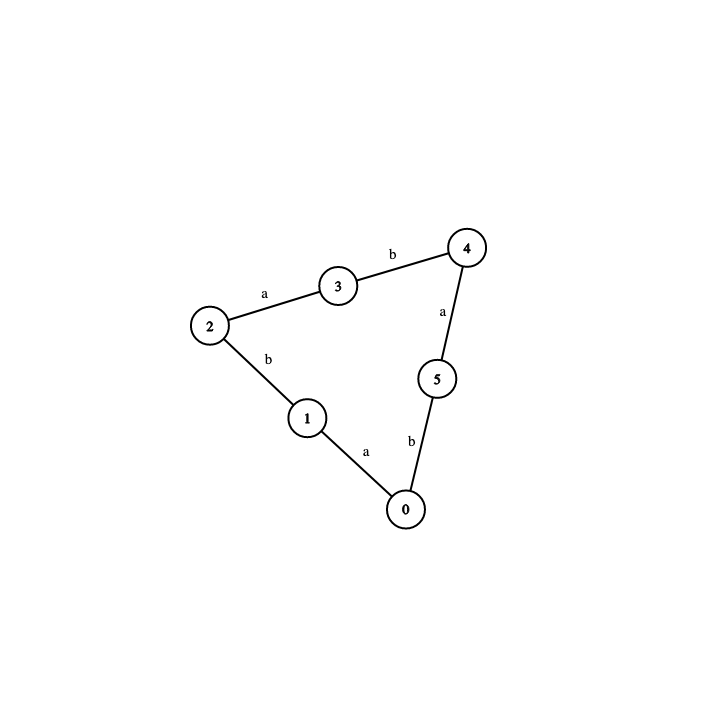
\includegraphics[width=0.5\textwidth]{figs/consistentlabelling-1.png}
	\caption{Illustration of consistent labelling.\label{fig:consistent-labeling-1}}
\end{figure}


\paragraph{Example} Figure \ref{fig:consistent-labeling-1} depicts a consistent edge labelling of the graph. 

\begin{definition}[Zig Zag Product]
	\label{def:zig zag product}
	\textbf{Input \& Output}
	\begin{equation}
		\left. \begin{aligned}
 			G: (N, D, -) \\
 			H: (D, D_1, -) 
 		\end{aligned}\right\rbrace \rightarrow G \tcircle{z} H : (ND, D_1^2, -)
	\end{equation}
	\textbf{Rotations}
	\begin{align}
		&\left. \begin{aligned}
 			Rot_G: [N] \times [D] \rightarrow [N] \times [D] \\
 			Rot_H: [D] \times [D_1] \rightarrow [D] \times [D_1]
 		\end{aligned}\right \rbrace 
 		\\
 		&\quad \quad \quad \quad \quad \quad
 		\rightarrow Rot_{G\tcircle{z} H}: [N\cdot D] \times \left( [D_1^2] \right) \rightarrow [N\cdot D] \times \left( [D_1^2] \right)
 		\\
 		&\quad \quad \quad \quad \quad \quad
 		\equiv Rot_{G\tcircle{z} H}: [N\cdot D] \times \left( [D_1] \times [D_1] \right) \rightarrow [N\cdot D] \times \left( [D_1] \times [D_1] \right)
	\end{align}
	and 
	\begin{align}
		&Rot_{G \tcircle {z}  H} \left ( (v, a) , (k_1, k_2) \right) : \\
		&\quad \rightarrow (a', i') \gets Rot_H(a, k_1) \\
		&\quad \rightarrow (w, b') \gets Rot_G (v, a') \\
		&\quad \rightarrow (b, i'') \gets Rot_H (b', k_2) \\
		&\quad \rightarrow \text{output} \left( (w, b), (k_2, k_1) \right)
	\end{align}
	\paragraph{English Explanation} The Zig-Zag product $G \tcircle{z} H$ replaces each vertex of $G$ with a copy (cloud) of $H$, and connects the vertices by moving a small step (zig) inside the cloud, followed by a big step between two clouds, and finally performs another small step (zag) inside the destination cloud. 
\end{definition}

\section{Zig Zag Analysis}
In the previous section, we highlighted a combinatorial product between two graphs called Zig Zag product. Here we present properties and analysis of the product. 

\paragraph{Goal} Consider the definition, where we are given graphs
\begin{equation}
	G: (N, D, \lambda_G) \quad \quad 
	\text{and} \quad \quad H : (D, D_1, \lambda_H)
\end{equation}
What can we tell about $G \tcircle {z} H$? In particular, it will be a $(ND, D_1^2, ??)$ graph? 

\begin{definition}[Tensor Product]
	For $A \in \real^{d_1 \times \d_1}$ and $B \in \real^{d_2 \times d_2}$, 
	\begin{equation}
		\real^{(d_1^2 )\times (d_2^2)} \ni A \otimes B \quad \text{where} \quad (A \otimes B)_{ij} = [A_{ij}B]
	\end{equation}
\end{definition}

\begin{proposition}[Adjacency of Zig Zag Product]
\label{prop:adjacency of zig zag product}
	For $F = G \tcircle {z} H$, 
	\begin{align}
		A_F 
		&= (\mathbb I _N \otimes A_H ) \cdot P_G \cdot ( \mathbb I _ N \otimes A_H ) \\
		&= \begin{bmatrix}
			[A_H] & [\bzero] & \dots & [\bzero] \\
			[\bzero] & [A_H] & \dots  & [\bzero] \\
			\vdots & \vdots & \ddots & [\vdots] \\
			[\bzero] & [\bzero] & \dots & [A_H]
		\end{bmatrix} \begin{bmatrix}
			[\dots] & [\dots] & \dots & [\dots] \\
			[\dots] & [\dots] & \dots  & [\dots] \\
			\vdots & \vdots & \ddots & [\vdots] \\
			[\dots] & [\dots] & \dots & [\dots]
		\end{bmatrix} \begin{bmatrix}
			[A_H] & [\bzero] & \dots & [\bzero] \\
			[\bzero] & [A_H] & \dots  & [\bzero] \\
			\vdots & \vdots & \ddots & [\vdots] \\
			[\bzero] & [\bzero] & \dots & [A_H]
		\end{bmatrix}
	\end{align}
	where each $[...]$ inside is of size $( D \times D)$, and thus the outer matrices are all of sizes $(D \times N) \times (D \times N )$. Graphically, we note that the two $(\mathbb I _N \otimes A_H )$ parts represent zig and zag steps respectively in the product while the $P$ transition is the inter-cloud big step.\footnote{A permutation transition $P$ guarantees that $P$ has only one 1 in each row and column. } 
	
	\paragraph{Normalized Adjacency}
	\begin{equation}
		M_F = A_F / D = (\mathbb I _N \otimes M_H ) \cdot P_G \cdot ( \mathbb I _ N \otimes M_H )
	\end{equation}
\end{proposition}

\begin{lemma}[Linear Algebra: LA1]
	\label{lemma: zig zag la 1}
	For $G$ is a $(N, D, -)$ graph, 
	\begin{equation}
		\lambda_G \leq \lambda \iff M_G = (1 - \lambda) \frac{J_N}{N} + \lambda \cdot E
	\end{equation}\footnote{$J_N$ is a box of $N \times N$ matrix, filled with 1's in every entry.}
	where \footnote{$\norm{ \cdot }$ is the spectral norm of a matrix, \textbf{and is equal to the largest absolute eigenvalue for a symmetric matrix.} }
	\begin{equation}
		\norm{ E } \leq 1
	\end{equation}
\end{lemma}

\paragraph{Remark} Consider spectral decomposition of $M_G$,
\begin{align}
	M_G 
	&= 1 \cdot \begin{bmatrix}
		1/\sqrt{n} \\ 1/\sqrt{n} \\ \vdots \\ 1/\sqrt{n}
	\end{bmatrix} \begin{bmatrix}
		\frac{1}{\sqrt{n}} & \frac{1}{\sqrt{n}} & \dots & \frac{1}{\sqrt{n}}
	\end{bmatrix} + \lambda_2 \bv_2 \bv_2^\top + \lambda_3 \bv_3 \bv_3^\top + \dots + \lambda_N \bv_N \bv_N^\top \\
	&= 1 \left( \frac{J_N}{N} \right) + \lambda_2 \bv_2 \bv_2^\top + \lambda_3 \bv_3 \bv_3^\top + \dots + \lambda_N \bv_N \bv_N^\top \\
	&= (1 - \lambda) \left( \frac{J_N}{N} \right) + \underbrace{\left( \lambda \left( \frac{J_N}{N} \right) + \lambda_2 \bv_2 \bv_2^\top + \lambda_3 \bv_3 \bv_3^\top + \dots + \lambda_N \bv_N \bv_N^\top \right)}_{E}
\end{align}
If fact this sum that we called $E$ is the Eigen decomposition of $E$ itself! 

\begin{lemma}[Linear Algebra LA 2]
\label{lemma: zig zag la 2}
	For $A, B \in \real^{N \times N}$,
	\begin{itemize}
		\item $\norm{ A + B } \leq \norm {A} + \norm {B}$
		\item $\norm {A \cdot B }  \leq \norm{A} \cdot \norm{B}$
		\item $\norm {A \otimes B} = \norm {A } \cdot \norm {B}$
	\end{itemize}
\end{lemma}

\begin{lemma}[Linear Algebra LA 3]
\label{lemma: zig zag la 3}
	For any permutation matrix (each row and column has exactly one non-zero) $P$, 
	\begin{equation}
		\norm {P} = 1
	\end{equation}
\end{lemma}

\begin{theorem}[Rozenmann-Vadhan 05, RVW 01]
	\label{thm:rozenmann vadhan 05 rvw 01}
	For 
	\begin{equation}
		G: (N, D, \lambda_G) \quad \quad 
		\text{and} \quad \quad H : (D, D_1, \lambda_H)
	\end{equation}
	$F = G \tcircle {z} H$ is a $(ND, D_1^2, \lambda_F)$-graph, where 
	\begin{equation}
		\lambda_F \leq 1 - (1 - \lambda_H) ^2 (1 - \lambda_G) 
	\end{equation}
	
	\paragraph{Alternatives} 
	\begin{align}
		& \lambda_F \leq 1 - (1 - \lambda_H) ^2 (1 - \lambda_G) \\
		\iff & (1 - \lambda_H)^2 (1 - \lambda_G) \leq 1 - \lambda_F \\
		\iff & Gap(H)^2 \cdot Gap(G) \leq Gap(F)
	\end{align}
\end{theorem}

\begin{proof}
	We start with writing out a complete form of $M_F$. Recall from earlier (Prop. \ref{prop:adjacency of zig zag product}) that 
	\begin{equation}
		M_F = (\mathbb I _N \otimes M_H ) \cdot P_G \cdot ( \mathbb I _ N \otimes M_H )
	\end{equation}
	By Lemma \ref{lemma: zig zag la 1}, we can derive
	\begin{equation}
		M_H = \left( ( 1- \lambda_H ) \frac{J_D}{D} + \lambda_H E_H \right) \quad\quad \text{where} \quad \norm{E_H} \leq 1
	\end{equation}
	Then, 
	\begin{equation}
		\mathbb I _ N \otimes M_H = ( 1- \lambda_H) \mathbb I _N \otimes \frac{J_D}{D} + \lambda_H \mathbb I_N \otimes E_H
	\end{equation}
	and thus
	\begin{align}
		M_F 
		&= \left(
			(1 - \lambda_H) \mathbb I_N \otimes \frac{J_D}{D} + \lambda_H \mathbb I_N \otimes E_H
		\right) \times P \times \left( 
			(1 - \lambda_H) \mathbb I_N \otimes \frac{J_D}{D} + \lambda_H \mathbb I_N \otimes E_H
		\right) \\
		&= ( 1- \lambda_H )^2 \left( \mathbb I _N \otimes \frac{J_D}{D} \right) \cdot P \cdot \left( \mathbb I _N \otimes \frac{J_D}{D} \right) \\
		& \quad \quad + (1 - \lambda_H) \lambda_H \underbrace{\left( \mathbb I _N \otimes \frac{J_D}{D} \right) \cdot P \cdot ( \mathbb I _N \otimes E_H )}_{E^{(1)}} \\
		& \quad \quad + \lambda_H ( 1-\lambda_H) \underbrace{(\mathbb I _N \otimes E_H ) \cdot P \cdot \left( \mathbb I _N \otimes \frac{J_D}{D} \right)}_{E^{(2)}}  \\
		& \quad \quad + \lambda_H^2 \cdot \underbrace{(\mathbb I _N \otimes E_H ) \cdot P \cdot (\mathbb I _N \otimes E_H )} _{E^{(3)}} \\
		&= ( 1- \lambda_H )^2 \left( \mathbb I _N \otimes \frac{J_D}{D} \right) P \left( \mathbb I _N \otimes \frac{J_D}{D} \right) + \underbrace{(1 - \lambda_H)\lambda_H E^{(1)} + \lambda_H(1 - \lambda_H) E^{(2)} + \lambda_H^2 E^{(3)}}_{E^{(4)}} \label{eq:zig zag expanded M_F}
	\end{align}
	
	Here, $\norm {E^{(1)}}, \norm {E^{(2)}}, \norm {E^{(3)}} \leq 1$ by applying Lemma \ref{lemma: zig zag la 2} multiple times. I present the proof for $\norm{E^{(1)}} \leq 1$ here.
 	\begin{align}
		\norm{E^{(1)}}
		&= \norm{ \left( \mathbb I _N \otimes \frac{J_D}{D} \right) \cdot P \cdot ( \mathbb I _N \otimes E_H ) } \\
		&\leq \norm{\mathbb I _N \otimes \frac{J_D}{D}} \cdot \norm{P} \cdot \norm{ \mathbb I _N \otimes E_H} \\
		&\leq 1 \cdot 1 \cdot 1 \\
		&\leq 1
	\end{align}
	
	Then, 
	\begin{align}
		\norm{E^{(4)}} 
		&\leq \norm{ (1 - \lambda_H) \lambda_H + \lambda_H (1 - \lambda_H) + \lambda_H ^2} \\
		&= (1 - \lambda_H) \lambda_H + \lambda_H (1 - \lambda_H) + \lambda_H ^2 \\ 
		&= 2 \lambda_H (1 - \lambda_H) + \lambda_H^2 \\
		&= 1 - (1 - \lambda_H)^2
	\end{align}
	\begin{mdframed}
		\paragraph{Summary of Above}
		\begin{align}
			M_F
			&= (\mathbb I _N \otimes M_H ) \cdot P_G \cdot ( \mathbb I _ N \otimes M_H ) \\
			&= (1 - \lambda_H)^2 \underbrace{\left( \mathbb I _N \otimes \frac{J_D}{D} \right) \cdot P \cdot \left( \mathbb I _N \otimes \frac{J_D}{D} \right)}_{\alpha} + E^{(4)} \label{eq:zig zag m_f expanded form with e4}
		\end{align}
		where 
		\begin{equation}
			\norm{E^{(4)}} \leq 1 - (1 - \lambda_H) ^2
		\end{equation}
	\end{mdframed}
	
	We can massage and transform this result with 
	\begin{align}
		\alpha 
		&= \frac{1}{D^2} ( \mathbb I _N \otimes J_D ) \cdot P \cdot ( \mathbb I _N \otimes J_D )  \\
		&= \frac{1}{D^2} \cdot A_G \otimes J_D \\
		&= \frac{A_G}{D} \otimes \frac{J_D}{D} \\
		&= M_G \otimes \frac{J_D}{D}
	\end{align}
	and plug back into Eq. \ref{eq:zig zag m_f expanded form with e4} to get
	\begin{equation}
		M_F = (1 - \lambda_H)^2 \left( M_G \otimes \frac{J_D}{D} \right ) + E^{(4)} \label{eq:zig zag M_f replaced form}
	\end{equation}
	
	Recall from Lemma \ref{lemma: zig zag la 1} that
	\begin{equation}
		M_G = (1 - \lambda_G) \cdot \frac{J_N}{N} + \lambda_G \cdot E_G \quad \quad \text{where} \quad \norm{E_G} \leq 1
	\end{equation}
	plugging this back into Equation \ref{eq:zig zag M_f replaced form}, we get 
	\begin{align}
		M_F
		&= (1 - \lambda_H) ^ 2 (1 - \lambda_G) \left( \frac{J_N \otimes J_D}{ND} \right) + (1 - \lambda_H ) ^2 \cdot \lambda_G \left( E_G \otimes \frac{J_D}{D} \right) + E^{(4)} \\
		&= (1 - \lambda_H)^2 (1 - \lambda_G) \frac{J_{ND}}{ND} + \underbrace{(1 - \lambda_H)^2 \cdot \lambda_G \cdot \left( E_G \otimes \frac{J_D}{D} \right) + E^{(4)}}_{E^{(5)}}
	\end{align}
	
	We can quantify $\norm{E^{(5)}}$ as 
	\begin{align}
		\norm{E^{(5)}}
		& \leq ( 1- \lambda_H)^2 \cdot \lambda_G \cdot \norm{E_G \otimes \frac{J_D}{D}} + \norm{ E^{(4)}} \\
		& \leq ( 1- \lambda_H)^2 \cdot \lambda_G \cdot 1 + 1 - (1 - \lambda_H) ^2 \\
		& = {1 - (1 - \lambda_G) \cdot (1 - \lambda_H) ^ 2}
	\end{align}
	
	\begin{mdframed}
		\paragraph{Summary of Above}
		\begin{equation}
			M_F = (1 - \mu) \cdot \frac{J_{ND}}{ND} + E^{(5)} \quad\quad \text{where} \quad \norm{E^{(5)}} \leq 1 - (1 - \lambda_G) \cdot (1 - \lambda_H) ^ 2
		\end{equation}
		i.e., the second largest eigenvalue of $M_F$ is at most $1 - (1 - \lambda_G) \cdot (1 - \lambda_H) ^ 2$ (by Lemma \ref{lemma: zig zag la 1}). 
	\end{mdframed}
	
	This concludes the proof. \qed
\end{proof}


\section{Undirected s-t Connectivity in Log Space}
\subsection{The Procedure}
\begin{algorithm}[USTCONN Log Space]
This is a four step procedure, with input $G = (V, E)$ and two nodes $s, t$ in the graph. We wish to output if $s, t$ are connected with each other. 

\begin{itemize}
	\item \textbf{Step 1.} Transform 
		\begin{equation}
			(G, s, t) \leadsto (G_0, s_0, t_0)
		\end{equation}
		where $G_0$ is a $B^2$ regular graph, for some constant $B$. \footnote{For example, we have the power to transform any graph into a 4-regular graph using the algorithm detailed previously.}
	\item \textbf{Step 2.} Fix $H$, a $(B^4, B, 1/4)$ graph. 
	\item \textbf{Step 3.} For $k \gets 1, \dots, L$, compute\footnote{Invariant: $G_k$ is always a $B^2$ regular graph. }\footnote{Remark: $|G_k| = N \cdot B^{4k}$. We than think of vertices in $G_k$ as $\bar v \equiv (v, a_1, a_2, \dots, a_k)$ where $v$ is a vertex in $G_0$ and $a_.$ is a vertex name in $H$. }
		\begin{equation}
			G_k = G_{k - 1}^2 \tcircle{z} H
		\end{equation}
	\item \textbf{Step 4.} Solve $s_{L}$, $t_{L}$ connectivity on $G_L$ by path enumeration.  
\end{itemize}	
\end{algorithm}

\subsection{Path Enumeration Path Length Analysis}
Let $\lambda_k$ denote the second largest eigenvalue of a connected component of $G_k$. We know from Thm. \ref{thm:rozenmann vadhan 05 rvw 01} that 
\begin{equation}
	\lambda_k \leq 1 - (1 - \lambda_H) ^ 2 \cdot ( 1- \lambda_{k - 1} ^2 ) 
\end{equation}
where we have $\lambda_{k - 1} ^2$ because $G_k = G_{k - 1}^2 \tcircle{z} H$. By assumption on $H$ that $\lambda_H \leq 1/4)$, 
\begin{align}
	&\lambda_k \leq 1 - \left( \frac{3}{4} \right) ^ 2 \cdot (1 - \lambda_{k - 1}^2 ) \\
	\implies & \left( \frac{3}{4} \right) ^ 2 ( 1 - \lambda_{k - 1}^2 ) \leq 1 - \lambda_k \\
	\implies & \left( \left ( \frac{3}{4} \right) \cdot ( 1 + \lambda_{k - 1} ) \right) ( 1 - \lambda_{k - 1} )  \leq (1 - \lambda_k) \\
	\implies & (1 - \lambda_k) \geq \min \left( \frac{1}{18}, \frac{35}{32} ( 1 - \lambda_{k - 1} ) \right )
\end{align}

\begin{proposition} 
If $L = \mathcal O (\log N_0 )$, then we will have 
\begin{equation}
	1 - \lambda_L \geq \frac{1}{18} \quad \quad \iff 
	\quad \quad \lambda_L \leq \frac{17}{18}
\end{equation}	
\end{proposition}

\begin{proposition}
	Path enumeration on $G_L$ results in paths of length 
	\begin{equation}
		\Delta = \mathcal O \left( \log _{\frac{1}{\lambda_L}} N_L \right) = \mathcal O \left( \log N_0 \right)
	\end{equation}
\end{proposition}
\begin{proof}
	By invariant stated above, 
	\begin{equation}
		N_L = N_0 \cdot B^{4L}
	\end{equation}
	then the path length bound becomes
	\begin{equation}
		\log _{\frac{1}{\lambda_L}} N_L \leq \log_{\frac{18}{17}} N_L \leq \mathcal O( \log N_0 ) + \mathcal (L )
	\end{equation}
\end{proof}


\subsection{Space Complexity}
\paragraph{Input} We are given the raw input graph $G_0$, original source and target $s_0, t_0$. Recall from earlier that we can label vertices in $G_L$ as
\begin{equation}
	(v\in G_0, a_1 \in V_H, a_2 \in V_H, \dots, a_L \in V_H)
\end{equation}
which is a path that we took from a vertex in $G_0$ via a series of steps labeled with vertices in $H$. 

\paragraph{Goal} Given a sequence of edge labels in $G_L$, 
$
	(e_1, e_2, \dots, e_\Delta)
$
we have to check where we end in $G_L$. 

\paragraph{Idea}
Recall that the original goal is to compute this query space efficiently. In particular, that means we don't have the luxury of computing out the entire $G_L$ graph. We can instead compute the rotation maps 
\begin{equation}
	Rot_{G_k}: [N_k] \times [B^2] \rightarrow [N_k] \times [B^2]
\end{equation}
recursively, following $G_k = G^2_{k - 1} \tcircle {z} H$. 

\paragraph{Recursive Computation}
Suppose we are to compute 
\begin{equation}
	Rot_{G_k}\left( (v, a_1, a_2, \dots, a_k) , e \in [B^2] \right)
\end{equation}
given $Rot_{G_{k - 1}}$. We can compute $Rot_{G^2_{k - 1} \tcircle {z} H}$ using the steps outlined in Definition \ref{def:zig zag product}. Unwinding, 
\begin{equation}
	Rot_{G^2_{k - 1}} \left( \bar v, ( f_1, f_2 ) \right) = Rot_{G_{k - 1}} \left( Rot_{G_{k - 1}} (\bar v, f_1 ) , f_2 \right)
\end{equation}
where $f_1, f_2$ are edge labels in $G_{k - 1}$. 

\paragraph{Space Complexity}
With some careful book keeping, we can implement the recursive procedure outlined above with a total of 
\begin{equation}
	\mathcal O (\log N )
\end{equation}
extra memory. 


\section{Expander Graphs}
\begin{definition}[Spectral Expander]
	A $D$-regular graph is a $\lambda$-expander if $G$ is a $(N, D, \lambda)$-graph.
\end{definition}

\paragraph{Example} Suppose that we have a $(N = 10^6, D = 10, \lambda \leq 1/2 )$-graph. Then, every two nodes in this graph are connected by a path of length $\leq \log D \log_{1/\lambda} N = \log 10 \log_{2} 10^6 \leq 24$. 

\begin{proposition}[Expander Graphs Properties]
	If $\lambda \leq \frac{1}{2}$, then for any set of nodes $S$ in this expander graph , the number of edges between $S$ and $\bar S$ is such that
	\begin{equation}
		E(S, \bar S) \geq \Omega (1) \cdot |S|
	\end{equation}
\end{proposition}

\begin{definition}[Expander Graph Intuitively]
	Expander Graphs = extremely well-connected graphs with few edges. 	
\end{definition}

\subsection{History of Expander Graphs}
The guiding question can be summarized as follows: (with example $D$ and $\lambda$ values 
\begin{quote}
	Given $N$, degree $D = 4$ and $\lambda = 0.9$. Can we find a $(M, D, \lambda)$-graph where $M \in (N, 20)$. 
\end{quote}

...
